\subsection{USB-B}
\label{subsec:USB-B}

Auf der Leiterplatte des PartyMixer's gibt es zwei Komponenten, welche programmiert werden müssen. Der Mikrocontroller und das WiFi-Modul. Um diese zu programmieren braucht es eine entsprechende Schnittstelle, welche mit einer USB-B-Schnittstelle realisiert wird.

Die USB-B-Schnittstelle benötigt nur zwei Kommunikationsleitungen (D+ und D-). Die zu programmierenden Komponenten (ESP32 und ATMega2560) benötigen zusätzliche Steuerleitungen um in einen Programmiermodus zu kommen und statt einem differenziellen Verfahrens ein serielles Verfahren. Deswegen wird ein USB-UART-Converter verwendet, welcher das Signal wandelt und die Steuerleitungen zur Verfügung stellt.

Die beiden Programmierschnittstellen (ATMega2560 und ESP32) benötigen unterschiedlich viele Steuerleitungen, da sie sich im Verfahren zum Aufruf des Download-Boot-Modus unterscheiden. In Tabelle \ref{tab:USB_uC} und \ref{tab:USB_ESP} wird dargestellt, welche Leitungen für das jeweilige Flash-Interface benötigt werden. Die Signalfolge, um den Programmier-Modus zu starten, wird in den Kapiteln \ref{subsubsec:Handshake_ATMega2560} und \ref{subsubsec:Handshake_ESP32} beschrieben.
%Die USB-B-seitige Schnittstelle wird an den Computer angeschlossen und muss nicht häher betrachtet werden.

\begin{table}[h!]
\center
\begin{tabular}{|c|lcl|c|}
\hline
\textbf{Mikrocontroller} & & & & \textbf{USB-Flash-Device} \\ \hline
RX & <== & direkt & === & TX  \\
TX & === & direkt & ==> & RX  \\
Reset & <== & Kondensator & === & DTR \\
\hline
\end{tabular}
\caption{Verbindung zwischen USB und Mikrocontroller.}
\label{tab:USB_uC}
\end{table}

\begin{table}[h!]
\center
\begin{tabular}{|c|lcl|c|}
\hline
\textbf{ESP} & & & & \textbf{USB-Flash-Device} \\ \hline
RX & <== & direkt & === & TX  \\
TX & === & direkt & ==> & RX  \\
EN & <== & über Transistor & === & RTS \\
IO\_0 & <== & über Transistor & === & DTR \\
IO\_13 & <== & über Widerstand & === & RTS \\
IO\_15 & <== & über Widerstand & === & CTS \\
\hline
\end{tabular}
\caption{Verbindung zwischen USB und ESP.}
\label{tab:USB_ESP}
\end{table}

%Um in den automatischen Programmiermodus zu kommen, muss folgender Handshake zwischen den Geräten stattfinden:


%Auch hier wurde vom Arduino Uno-Board abgekpufert und der selbe Chip verwendet, um die USB-Signale in UART-Signale zu konvertieren. Das vorkommende Bauteil ist der CP2102N. Da dieser Chip ein TQFP-28-Gehause hat, könnte es auch schwierigkeiten geben beim Löten. Deswegen wird auch ein Breakout-Board (BOB) mitgeplant, damit es eine Ausweichmöglickeit gibt falls die Bauteile zu klein sind.

%\begin{figure}[!h]
%\center
%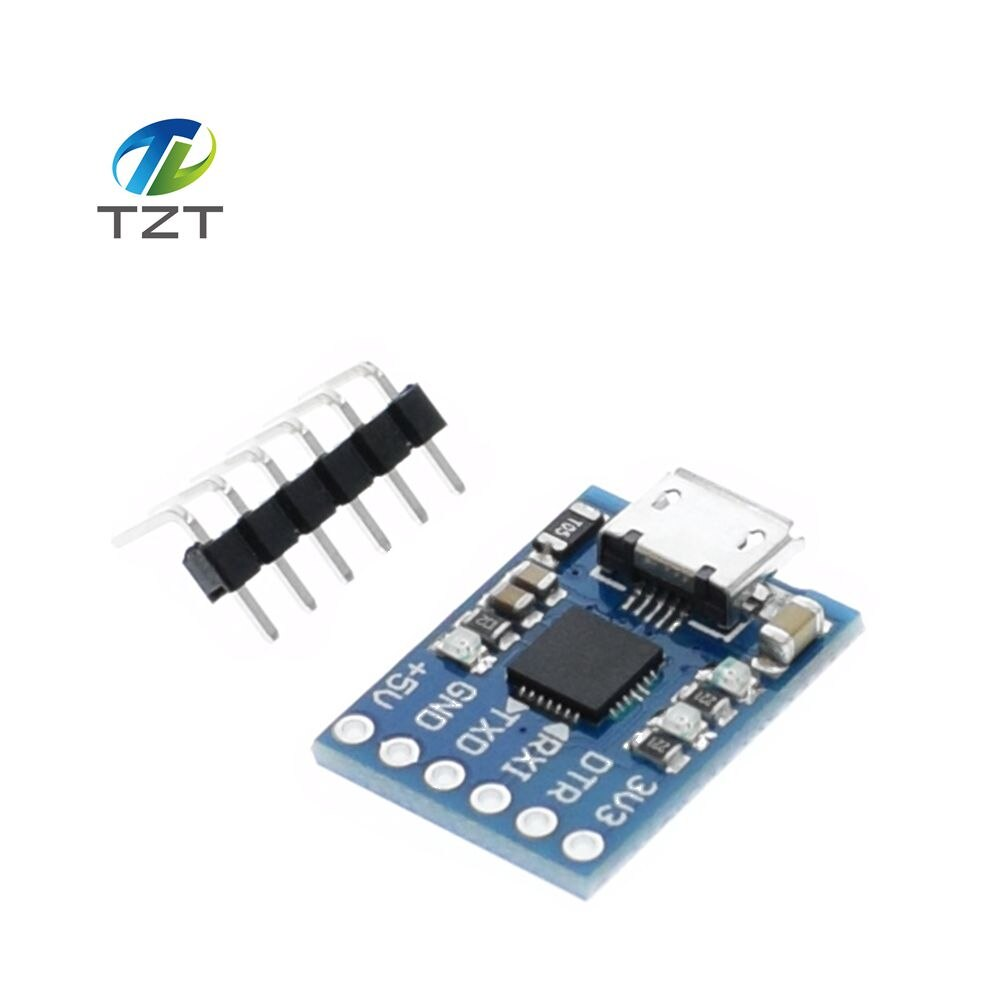
\includegraphics[width = 0.5\textwidth]{graphics/Produktbild_USB_UART_uC}
%\caption{CP2102N-BOB für uC.}
%\label{fig:Produktbild_USB_UART_uC}
%\end{figure}
%
%\begin{figure}[!h]
%\center
%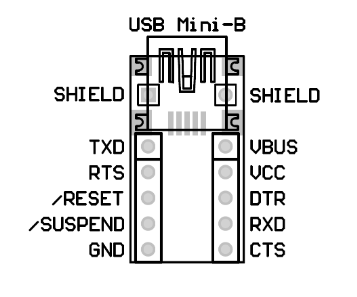
\includegraphics[width = 0.5\textwidth]{graphics/Produktbild_USB_UART_ESP}
%\caption{CP2102N-BOB für ESP.}
%\label{fig:Produktbild_USB_UART_ESP}
%\end{figure}
\subsubsection{Handshake ATMega2560}\label{subsubsec:Handshake_ATMega2560}

Der Handshake zwischen Computer und ATMega2560 ist einfacher zu verstehen als der Handshake zwischen Computer und ESP32. Da für den ATMega2560 ein stk500v2-Bootloader verwendet wird, erwartet dieser nur ein Flankenwechsel am Reset-Pin. Dadurch wird automatisch der im Programmspeicher abgelegte Bootloader gestartet und auf einkommende Daten gewartet. Nachdem das Programmiertool AVRdude die Device-Signatur (0x1E9801) verifiziert hat, sendet es das kompilierte HEX-File an den ATMega2560.

Um die Daten hochladen zu können, muss sichergestellt werden, dass avrdude mit dem stk500v2 programmer hochlädt und die DTR-Leitung toggelt, bevor der Programmiervorgang stattfindet. Die DTR-Leitung hängt über einen Kondensator an der Reset-Leitung und zieht diese auf GND, womit der Bootloader des ATMega2560 aktiv wird. Deswegen wird beim Hochladen in AVRdude als programming-id der \textit{wiring}-programmer angegeben, sichtbar in Kapitel \ref{subsubsec:avrdude_in_atmelstudio_einbinden} Tabelle \ref{tab:AVRdude_commands} (-c wiring).

\newpage

\subsubsection{Handshake ESP32}\label{subsubsec:Handshake_ESP32}
Nach einem Neustart des ESP32 werden die Zustände der Strapping-Pins gelesen. Anhand dieser Zustände werden die Grundzustände des ESP32 gesetzt, bevor der Programmcode gestartet wird. Anhand der Strapping-Pins wird auch der Download-Boot-Modus gestartet.
Um den Handshake zwischen Computer und ESP32 zu verstehen, muss zuerst Tabelle \ref{tab:Einfluss_Pins_auf_Boot_Modus} betrachtet werden, worin die Strapping-Pins aufgelistet sind und welchen Einfluss diese auf denn Boot- oder Download-Modus haben. Aufgrund der defaultmässigen Pull-up und -down Widerstände kann aus dieser interpretiert werden, dass wenn U0TXD, IO2 und IO5 ''floating'' sind, IO0 den Boot-Modus bestimmt.

\begin{table}[h!]
\center
\begin{tabular}{|l|c|c|c|}
\hline
\multicolumn{4}{|c|}{\textbf{Boot-Mode Konfiguration}}\\
\hline
\textbf{Pin} & \textbf{Default} & \textbf{Boot} & \textbf{Download} \\
\hline
IO0 & 1 & 1 & 0 \\
\hline
U0TXD & 1 & 1 & Don't care \\
\hline
IO2 & 0 & Don't care & 0 \\
\hline
IO15 & 1 & Don't care & Don't care \\
\hline
IO5 & 1 & 1 & Don't care \\
\hline
\end{tabular}
\caption{Wenn U0TXD, IO2, IO5 floating sind, bestimmt IO0 den Boot-Modus.}
\label{tab:Einfluss_Pins_auf_Boot_Modus}
\end{table}

Im Getting Started Guide vom ESP32 steht geschrieben, dass wenn während die beiden Pins IO0 und EN GND gezogen werden, das Modul in den Download-Modus versetzt wird, die Firmware über den UART-Port herunterlädt und diese in den Flash-Speicher schreibt. Um dies über die DTR- und RTS-Leitung machen zu können, braucht es eine zusätzliche Programmierlogik.

Mit der Schaltung, wie sie in Abbildung \ref{fig:Schema_ESP32_Flashbuttons} ersichtlich ist, kann das ESP32-Modul mit einer bestimmten Signalabfolge an den Leitungen DTR und RTS in diesen Download-Boot-Modus gesetzt werden. Die Auswirkung der Schaltung auf IO0 und den EN-Pin kann in Tabelle \ref{tab:Einfluss_Boot_Schaltung} entnommen werden.

\begin{table}[h!]
\center
\begin{tabular}{|c|c||c|c|}
\hline
\multicolumn{4}{|c|}{\textbf{Auto Program Cirquit}}\\
\hline
\textbf{DTR} & \textbf{RTS} & \textbf{EN} & \textbf{IO0} \\
\hline
1 & 1 & 1 & 1 \\
\hline
0 & 0 & 1 & 1 \\
\hline
1 & 0 & 0 & 1 \\
\hline
0 & 1 & 1 & 0 \\
\hline
\end{tabular}

\caption{Strapping pins des ESP32 und deren Auswirkung auf den Boot- und Download-Modus beim aufstarten.}
\label{tab:Einfluss_Boot_Schaltung}
\end{table}

Die Programmierlogik wird aus dem Programmiertool angesteuert. Es befindet sich in der ESP-Bibliothek, welche verwendet wird, um Code aus der Arduino-Umgebung hochzuladen. Aus dem Python-Skript kann entnommen werden, wie die Pins angesteuert werden. Der Code ist in Abbildung \ref{fig:ESP32_Boot_Code} dargestellt.\\
Bei der Interpretation des Codes ist darauf zu achten, dass die beiden Pins DTR und RTS Active-Low sind. (True = 0V = 0 = LOW und False = VCC = 1 = HIGH). Der Bezug zwischen dem Upload des Programms, den Pins des ESP32 und dessen Download-Boot-Modus sowie den Leitungen DTR und RST wird in Tabelle \ref{tab:Abfolge_Download_Boot_Modus} aufgezeigt.
%Daraus erkennbar ist, dass:
%\begin{table}
%\begin{tabular}{lll}
%DTR & RTS & Status\\
%1 & 0 & Reset\\
%1 & 1 & Starte Run-Modus\\
%1 & 0 & IO0 = 0\\
%0 & 0 & Starte Run-Modus\\
%\hline
%\end{tabular}
%\end{table}
\todo{Referenz einfügen: http://loboris.eu/ESP32/ESP32\_AutoReset.jpg}


\newpage
\begin{figure}[h!]
	\centering
	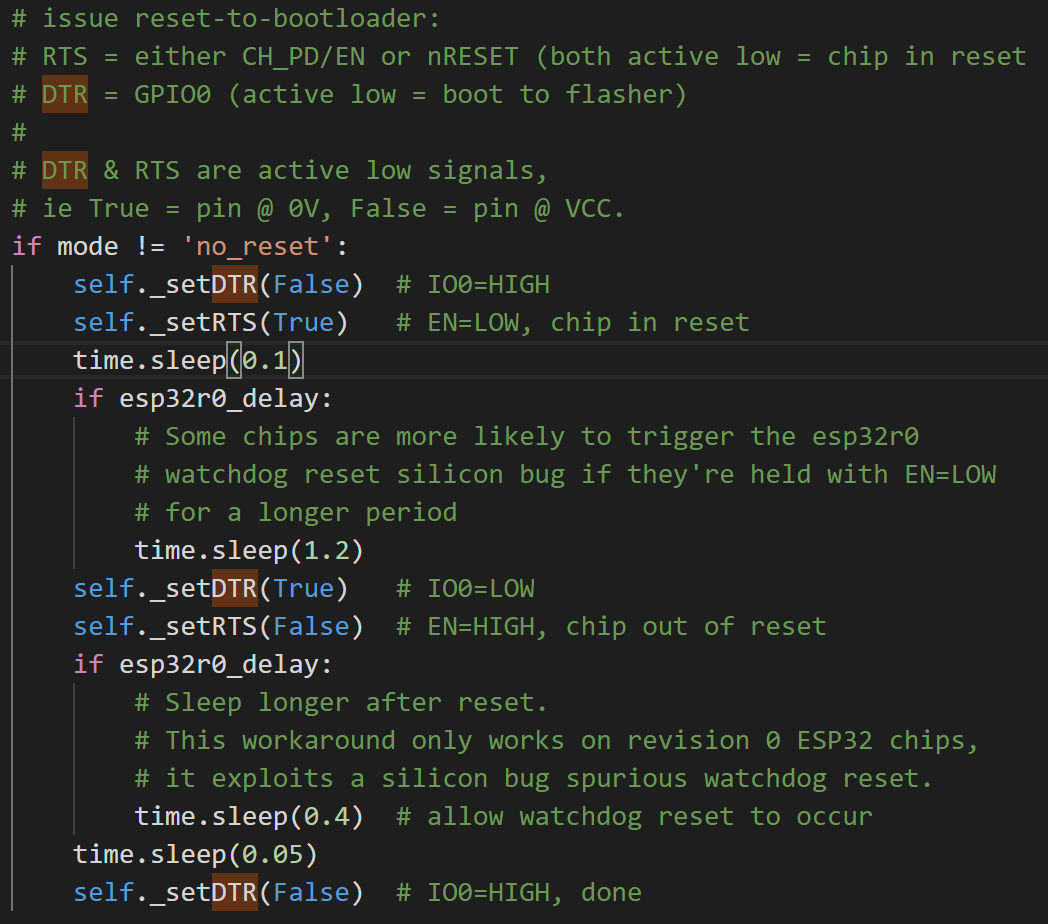
\includegraphics[width=0.8\textwidth]{graphics/ESP32_Boot_Code}
	\caption{Codeausschnitt aus dem Programmier-Tool. Auf diese Weise werden der DTR- und der RTS-Pin angesteuert während dem Programmiervorgang.}
	\label{fig:ESP32_Boot_Code}
\end{figure}

\begin{table}[h!]
\center
\begin{tabularx}{\textwidth}{|l|X||c|c||c|c|}
\hline
Schritt & Beschreibung & DTR & RTS & EN & IO0\\
\hline
1 & Im ersten Schritt wird der Chip mit \textit{EN = 0} und \textit{IO0 = 1} in den Reset-Modus geschaltet und im Programm 0.1ms gewartet. & 1 & 0 & 0 & 1 \\
\hline
2 & Im zweiten Schritt werden die Zustände geändert, jetzt ist \textit{EN = 1} und \textit{IO0 = 0} \textit{IO0 = 0}. Aufgrund der Kapazität am EN-Pin wird die Spannung für einen kurzen Moment tief gehalten. Dies hat Schritt 3 zur Folge. & 0 & 1 & 1 & 0 \\
\hline
3 & Die durch den Kondensator C7 tief gehaltene Spannung bewirkt, dass sich die Zustsände über den Pins wie folgt verhalten: \textit{EN = 0} und \textit{IO0 = 0}. Im Programm wird 0.05ms gewartet. Danach ist das ESP32 im Download-Boot-Modus und das zu speichernde Programm kann hochgeladen werden. & 0 & 1 & 0 & 0 \\
\hline
4 & Nachdem das Programm hochgeladen wurde, werden beide Zustände auf 1 gesetzt. Das ESP32 startet nun den neu hochgeladenen Programmcode. & 1 & 1 & 1 & 1 \\
\hline
\end{tabularx}
\caption{Abfolge der Schritte während dem Aufrufen des Download-Boot-Modus.}
\label{tab:Abfolge_Download_Boot_Modus}
\end{table}
